\documentclass[border=4pt]{standalone}
\usepackage[T1]{fontenc}
\usepackage{lmodern}
\usepackage{amsmath}
\usepackage{tikz}
\usetikzlibrary{positioning,arrows.meta,fit,backgrounds,calc}
\begin{document}
\sffamily\footnotesize
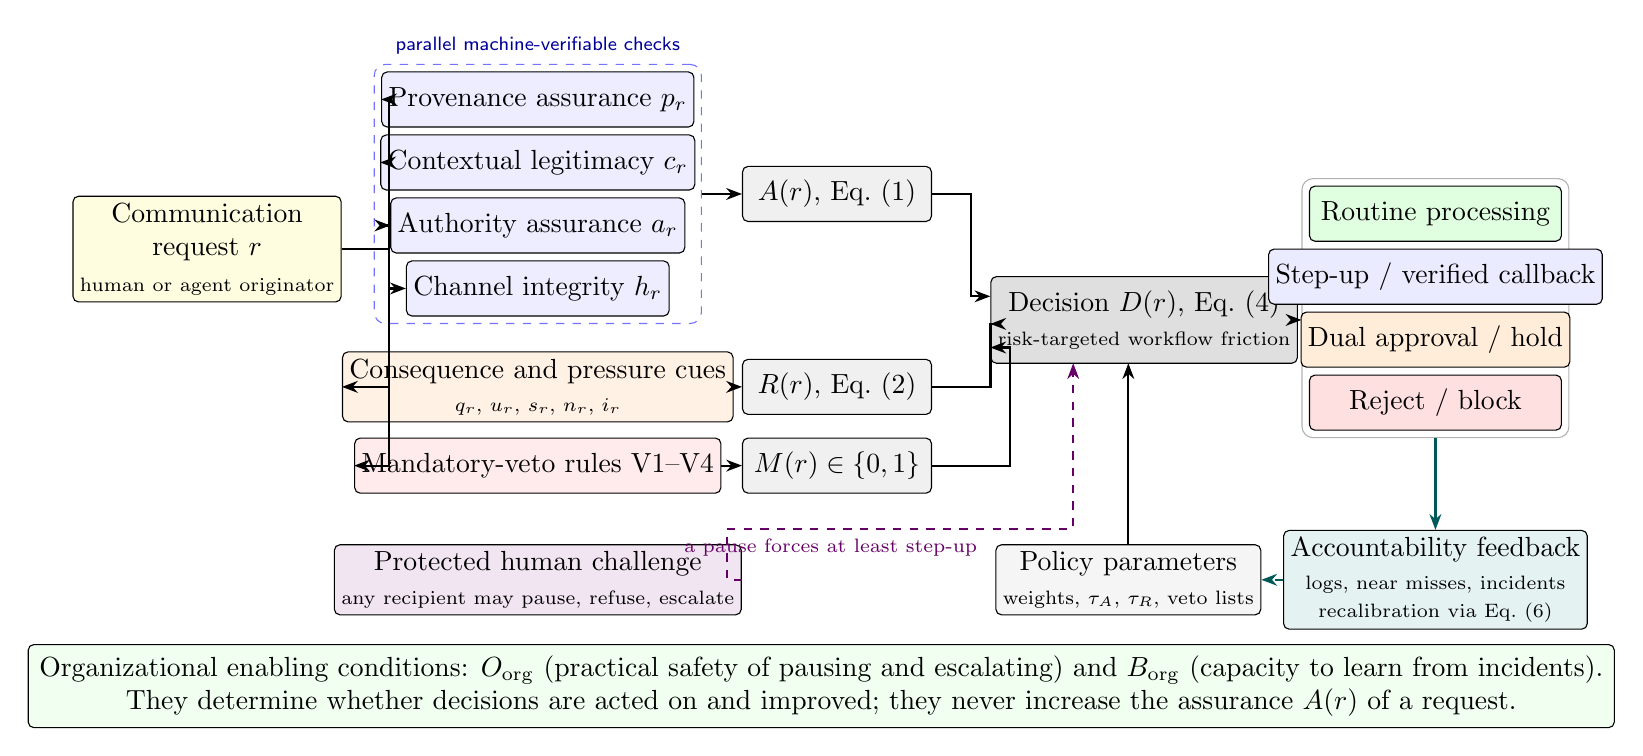
\begin{tikzpicture}[
  box/.style={draw, rounded corners=2pt, align=center, minimum height=7mm, inner sep=2.5pt, fill=white},
  chk/.style={box, fill=blue!7, minimum width=33mm},
  agg/.style={box, fill=gray!12, minimum width=24mm},
  oc/.style={box, minimum width=32mm},
  arr/.style={-{Stealth[length=2mm]}, thick},
  dsh/.style={-{Stealth[length=2mm]}, thick, dashed}
]
% column 1: request
\node[box, fill=yellow!12, minimum width=26mm] (req) at (0,0.5) {Communication\\request $r$\\[1pt]{\scriptsize human or agent originator}};
% column 2: evidence and pressure inputs
\node[chk] (p) at (4.2, 2.4) {Provenance assurance $p_r$};
\node[chk] (c) at (4.2, 1.6) {Contextual legitimacy $c_r$};
\node[chk] (a) at (4.2, 0.8) {Authority assurance $a_r$};
\node[chk] (h) at (4.2, 0.0) {Channel integrity $h_r$};
\begin{scope}[on background layer]
\node[draw=blue!55, dashed, rounded corners, fit=(p)(h), inner sep=2.5pt, label={[font=\scriptsize\sffamily, text=blue!60!black]above:parallel machine-verifiable checks}] (par) {};
\end{scope}
\node[box, fill=orange!10, minimum width=33mm] (pr) at (4.2,-1.25) {Consequence and pressure cues\\{\scriptsize $q_r$, $u_r$, $s_r$, $n_r$, $i_r$}};
\node[box, fill=red!8, minimum width=33mm] (vt) at (4.2,-2.25) {Mandatory-veto rules V1--V4};
% column 3: aggregation
\node[agg] (A) at (8.0, 1.2) {$A(r)$, Eq.~(1)};
\node[agg] (R) at (8.0,-1.25) {$R(r)$, Eq.~(2)};
\node[agg] (M) at (8.0,-2.25) {$M(r)\in\{0,1\}$};
% column 4: decision
\node[box, fill=gray!25, minimum width=30mm, minimum height=11mm] (D) at (11.9,-0.4) {Decision $D(r)$, Eq.~(4)\\{\scriptsize risk-targeted workflow friction}};
% column 5: outcomes
\node[oc, fill=green!12] (o1) at (15.6,0.95) {Routine processing};
\node[oc, fill=blue!8]   (o2) at (15.6,0.15) {Step-up / verified callback};
\node[oc, fill=orange!15](o3) at (15.6,-0.65) {Dual approval / hold};
\node[oc, fill=red!12]   (o4) at (15.6,-1.45) {Reject / block};
\begin{scope}[on background layer]
\node[draw=gray!60, rounded corners, fit=(o1)(o4), inner sep=2.5pt] (outs) {};
\end{scope}
% bottom row
\node[box, fill=violet!10, minimum width=33mm] (hc) at (4.2,-3.7) {Protected human challenge\\{\scriptsize any recipient may pause, refuse, escalate}};
\node[box, fill=gray!8, minimum width=27mm] (pm) at (11.7,-3.7) {Policy parameters\\{\scriptsize weights, $\tau_A$, $\tau_R$, veto lists}};
\node[box, fill=teal!10, minimum width=32mm] (fb) at (15.6,-3.7) {Accountability feedback\\{\scriptsize logs, near misses, incidents}\\[-2pt]{\scriptsize recalibration via Eq.~(6)}};
% arrows: inputs
\foreach \n in {p,c,a,h,pr,vt} \draw[arr] (req.east) -- ++(6mm,0) |- (\n.west);
\draw[arr] (par.east) -- ++(4mm,0) |- (A.west);
\draw[arr] (pr.east) -- (R.west);
\draw[arr] (vt.east) -- (M.west);
\draw[arr] (A.east) -- (9.7,1.2) |- ($(D.west)+(0,0.3)$);
\draw[arr] (R.east) -- (9.95,-1.25) |- ($(D.west)+(0,-0.05)$);
\draw[arr] (M.east) -- (10.2,-2.25) |- ($(D.west)+(0,-0.35)$);
\draw[arr] (D.east) -- (outs.west |- D.east);
% human challenge, feedback loop
\draw[dsh, violet!80!black] (hc.east) -- (6.6,-3.7) -- (6.6,-3.05) -- node[below, font=\scriptsize, text=violet!80!black, pos=0.3]{a pause forces at least step-up} (11.0,-3.05) -- (11.0,-0.95);
\draw[arr, teal!70!black] (outs.south) -- (fb.north);
\draw[dsh, teal!70!black] (fb.west) -- (pm.east);
\draw[arr] (pm.north) -- (11.7,-0.95);
% organisational band
\node[draw, rounded corners=2pt, fill=green!6, minimum width=172mm, align=center, inner sep=4pt] (org) at (7.8,-5.05)
 {Organizational enabling conditions: $O_{\mathrm{org}}$ (practical safety of pausing and escalating) and $B_{\mathrm{org}}$ (capacity to learn from incidents).\\ They determine whether decisions are acted on and improved; they never increase the assurance $A(r)$ of a request.};
\end{tikzpicture}
\end{document}
